\clearpage
\section{瓦力重复上一句，开口也慢}

玩家说「你好，我叫青桐。你叫什么名字？」旧版瓦力先报出自己的名字，又说看见玩家穿了一件旧工装。接着问「我刚告诉你我叫什么名字？」，它把整段台词又念了一遍。回放里两次模型输出完全相同。场景没有提供玩家穿工装的记录。这句话是模型第一次答话时编出来的，后来又进入了交谈记录。

新版先判断玩家在问什么。聊维修站时，瓦力读到的观察包括砂石路和旧油桶。核对姓名时，它读最近几轮对话的原文，每句话都注明是谁说的。这样就能从玩家说过的话里找到「青桐」。问考试时，它可以直接回应那件烦心事。换一个话题后，不再反复把场景里的工作和设备塞进回答。

\begin{center}
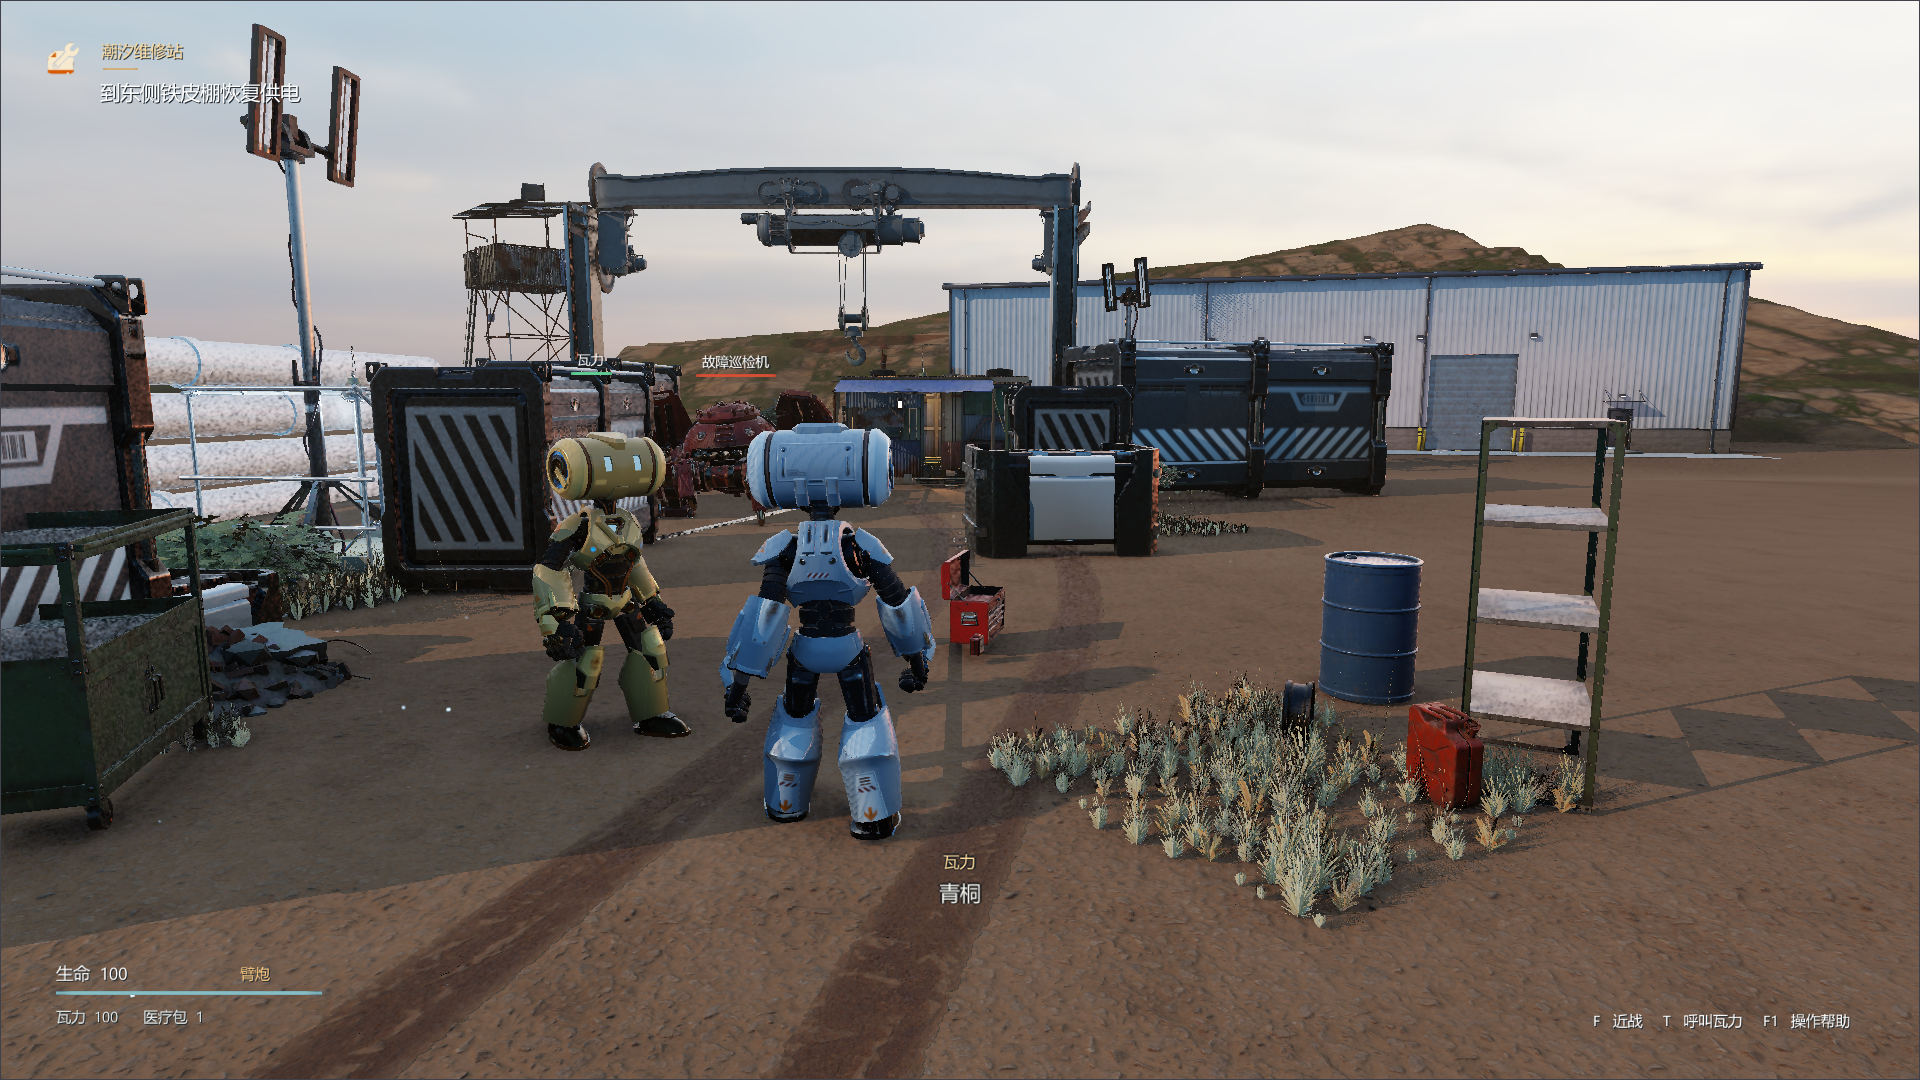
\includegraphics[height=6.8cm,trim=405bp 115bp 565bp 230bp,clip]{../../../output/validation/wali-conversation/recall.png}
\end{center}
\note{发行包实机画面局部。蓝灰色角色由玩家操作，左侧的瓦力开口说「青桐」，下方字幕显示本轮回答。}

玩家等的是声音。测试从游戏收到输入开始计时，直到 Windows 播放设备读到第一个有声采样。以前要等整段台词合成完。现在进入关卡时就开始加载 Dylan 音色，合成器每生成一小段声音，播放器就可以把它送给声卡。下表取自同一台电脑上的维修站发行包，单位为秒。

\smallskip
\noindent\begin{tabularx}{\linewidth}{Yrr}
\toprule
操作 & 旧版 & 新版 \\
\midrule
语音服务刚启动就问瓦力名字 & 62.99 & 33.58 \\
音色已经载入，追问玩家的名字 & 16.34 & 1.64 \\
音色已经载入，问维修站有什么印象 & 11.88 & 1.75 \\
音色已经载入，说起考试失利 & 14.84 & 2.64 \\
\bottomrule
\end{tabularx}

首次启动时，声音模型加载了约 40 秒，其中一部分与进入关卡重叠。再次开游戏时，启动器会寻找已在运行的语音服务。这一次四轮都在 2.64 秒内开口。每题各测了一次，完整原话、实际模型输入和声卡记录见 \path{output/validation/wali-conversation/}。
